\section{Introduction}


The ATLAS physics program relies on an efficient trigger system~\cite{aad2020performance} to record a highly signal-rich subset of all collision events produced by the Large Hadron Collider (LHC) at CERN. Electron triggers\cite{aaboud2019electron} are important for searches for new particles, the measurement of Standard Model cross-sections, and in the precise measurement of the properties of fundamental particles such as the Higgs~\cite{HIGG-2012-27,HIGG-2016-33} and W bosons.

A hierarchical two-level trigger system is used to select events with electrons produced by the LHC collisions. The first-level (L1) trigger, implemented with custom-made electronics located on the detector, utilises coarser granularity from the calorimeters to reduce the event rate from 40 MHz bunch crossing rate to below 100 kHz, of which about 35\% correspond to events with high-energy electromagnetic showers, potentially coming from electrons. The L1 level also defines regions-of-interest (RoIs)~\cite{CERN-LHCC-2017-020}, situated around local regions with high transverse energy. 

The RoIs accepted by L1 are processed by the HLT, based on algorithms implemented in software. The HLT operates from a large computing farm and should reduce the number of events written to disk to an average rate about 1 kHz.
For electron selection, the HLT is split into two stages: a fast but efficient computation followed by a precise processing, which employs offline inspired algorithms that are adapted to the harsh conditions (e.g., time and memory constraints) of the trigger system.  The HLT selection starts with the fast calorimeter reconstruction step (FastCalo), which has two implementations: an original cut-based algorithm and a new neural network approach based on the ring sums (Neural-Ringer algorithm), presented in this paper (Figure~\ref{fig:electron_chain}). 
This processing step is followed by the fast track reconstruction (FastElectron), which applies restrictions on variables that indicate the quality of proximity matching between the electron candidate positions reconstructed from the track and the calorimeter. The selection of particle candidates by the HLT is performed at each step, so that if it fails at a certain step, subsequent steps are not executed. This is essential to reduce the CPU resources and time needed by the HLT to reconstruct the event and make a decision. 


\begin{figure}[h!tb]
  \centering
  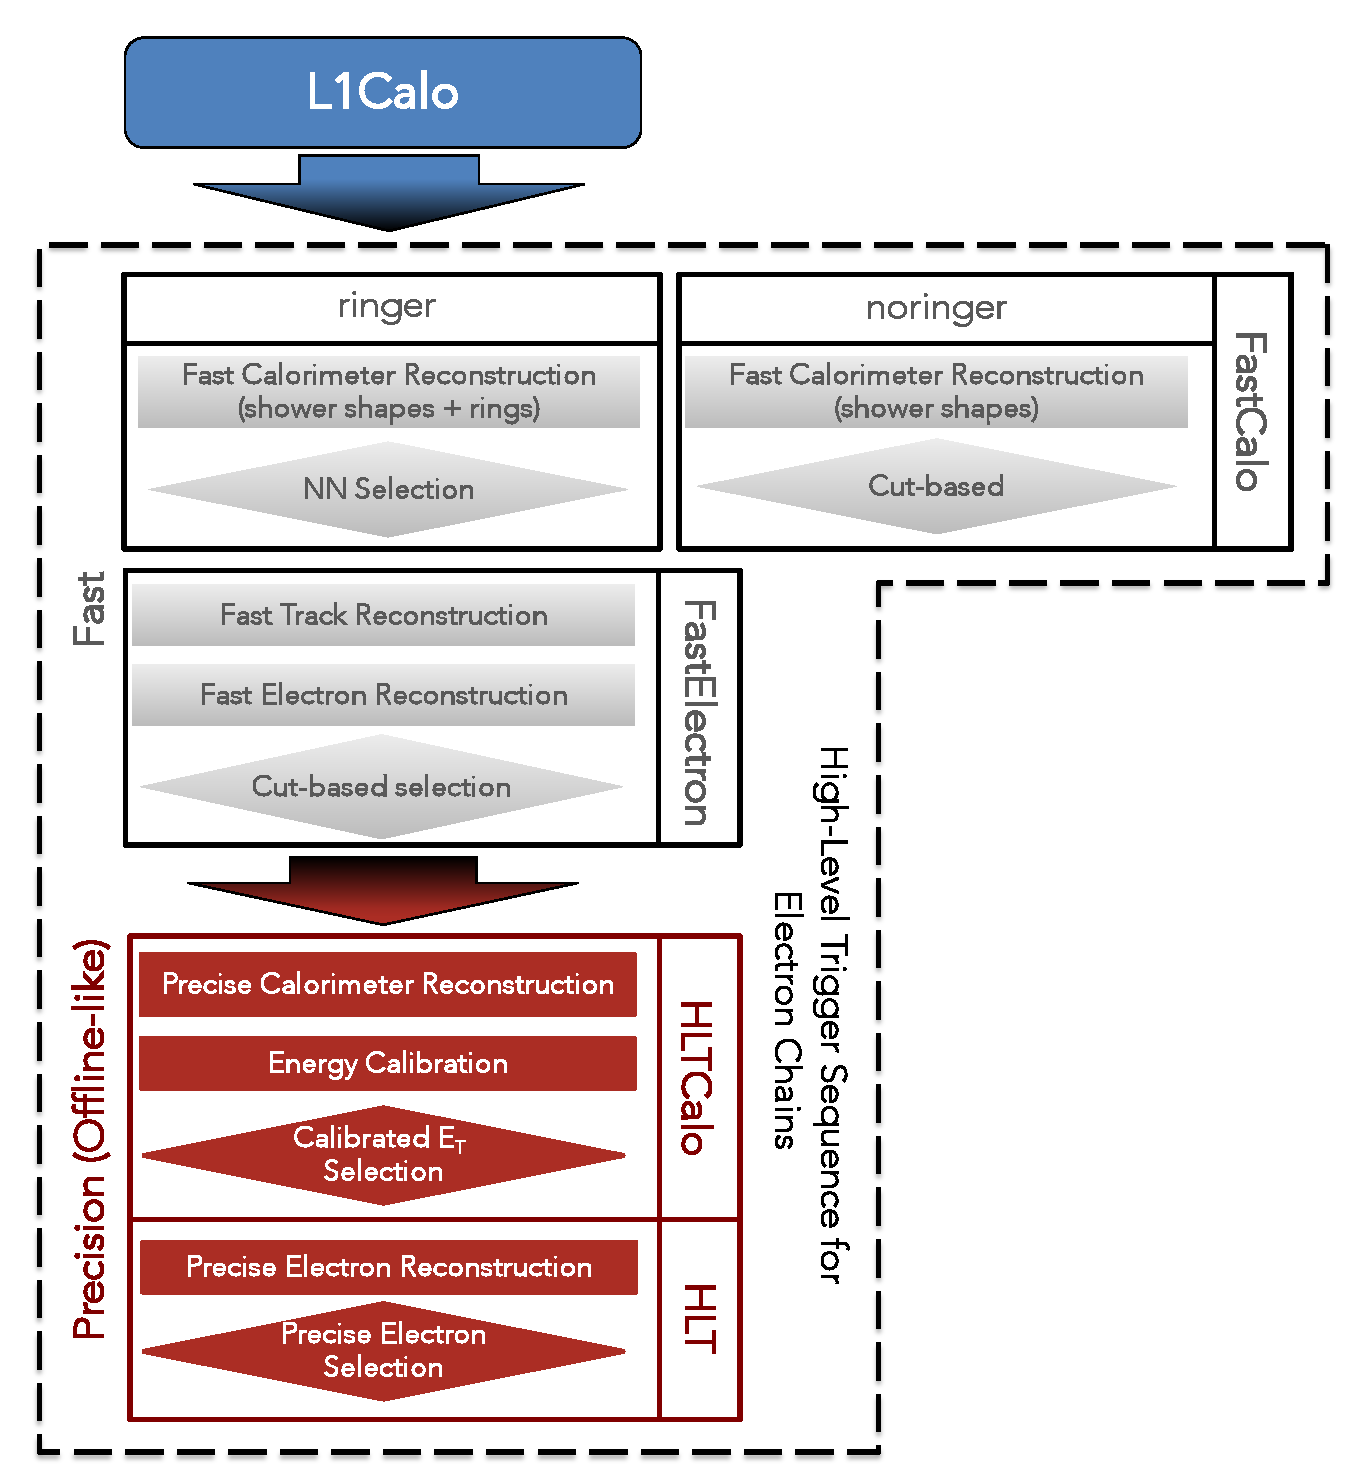
\includegraphics[width=0.7\textwidth]{sections/01_introduction/figures/ElectronChain_Run2_noringer_and_ringer.pdf}
  \caption{Comparison of the processing flow diagrams for the electron triggers with the logic employed in the triggers based on the cut-based strategy and the primary electron
  chains (ringer chains) since 2017, with the \rnn{} algorithm. The algorithms responsible for extracting some features from the event (also known as feature extraction) are represented by the red or gray rectangles. On the other hand, the algorithms responsible for making the decision to proceed to the next stage or not (called as hypothesis tests) are represented by the red or gray diamonds.}
  \label{fig:electron_chain}
\end{figure}




This paper describes the performance improvements due to introduction of the Neural-Ringer algorithm into the HLT fast calorimenter reconstruction step of the electron triggers, which became the baseline selection of events containing at least one isolated electron above 15 GeV in the 2017 proton-proton collision ATLAS data-taking. The Full details of its identification procedure are in Section~\ref{sec:neuralringer}, including the training and tuning strategies. The online performance results from the \rnn and the cut-based strategies are presented in Section~\ref{sec:operation} . A comparison of the \rnn with the cut-based triggers using statistical methods through the offline perspective is performed in Section~\ref{sec:off_ana}. Finally, the conclusions and prospects 
are derived in Section~\ref{sec:conclusion}.
